%----------------------------------------------------------------------------------------
% CHAPTER ONE
%----------------------------------------------------------------------------------------


\chapter{INTRODUCTION }
\label{ch:introduction}
In the conventional understanding of linear optics, the response of a material to an incident
electromagnetic wave is linearly proportional to the strength of the electric field. However, when
the intensity of the incident light becomes strong enough, the nonlinear optical response
becomes significant. This regime reveals a rich variety of phenomena, including the photoncarrier
injection, phase modulation, and harmonic generation.
After the first observation of nonlinear optical phenomena by Franken~\cite{franken1961generation},
based on recent advancements in laser technology, groundbreaking research in the field of nonlinear
optics have been driven~\cite{RevModPhys.72.545, RevModPhys.81.163, MOUROU2012720}, have conducted in a new era of intense light generation. These developments have paved the way for in-depth exploration of light-matter interactions in highly nonlinear regimes both in atomic and condensed matter phases. One of the most captivating nonlinear optical phenomena made accessible by these advances is High-order Harmonic Generation (\gls{HHG}), a process characterized by its extreme photon upconversion and remarkable nonlinear characteristics.

This thesis aims to provide a comprehensive overview of the nonlinear response phenomenons
including photocarrier injection and high-order harmonic generation from a theoretical point of view linked to the microscopic modeling of the electron dynamics in those 2d quantum materials. We will explore the theoretical foundations of light induced time-dependent quantum
dynamics evolution in solid systems,
including the quantum mechanical description of the light-matter ineraction process and the role of
excited electron dynamics.  By investigating photocarrier injection and HHG, we seek to deepen our understanding of the nonlinear optical response of materials and unlock the potential for applications in fields such as ultrafast spectroscopy, attosecond science, and advanced imaging techniques.
%=====================================================================================================================================
\section{Nonlinear Optical Response}
In studies of optical response theory within solid systems, the dielectric function serves as an centered concept, the dielectric function characterizes how the material's polarization, induced by the external field, evolves with the field's frequency and intensity. Mathematically, the dielectric function connects the material's polarization density to the electric field through Maxwell's equations, forming the basis for understanding its optical properties. Linear response theory, predicated on the assumption of weak perturbations, asserts that the induced polarization is directly proportional to the strength of the applied field.
Linear response theory is most applicable when the perturbations are weak. In other words, the system's behavior is approximately linear in the vicinity of its equilibrium or initial state.
In such cases. the system's behavior is described by linear susceptibility ($\chi^{(1)}$).

The electric susceptibility ($\chi^{(1)}$) describes the response of a material to an applied electric field ($\mathbf{E}$). The relationship between the induced polarization ($\mathbf{P}$) and the applied electric field can be expressed as:

\begin{equation}
	\mathbf{P^{(1)}(t)} =\epsilon_0 \int_{0}^{\infty}\mathbf R^{(1)} \cdot \mathbf{E}(t-\tau)d\tau
	\label{eqn:linearresponse}
\end{equation}
Where:
\begin{itemize}
	\item $\mathbf{P}$ is the induced polarization vector,
	\item $\mathbf R^{(1)}$ is the linear response function, electric susceptibility tensor, and
	\item $\mathbf{E}$ is the applied electric field vector.

\end{itemize}
Equation.~(\ref{eqn:linearresponse}) can be transformed to the frequency domain by intoducing the
Fourier trasnform of electric field:
\[
	E(\omega) =\int_{-\infty'}^{\infty}E(t) \cdot e^{i\omega t} dt.
\]
\[
	E(t) =\frac{1}{2\pi}\int_{-\infty'}^{\infty}E(\omega) \cdot e^{-i\omega t} d\omega.
\]
By introducing above Fourier transform, we have:
\[
	\mathbf P^{(1)}(t) =\epsilon_0 \int_{-\infty}^{\infty} \frac{d\omega}{2\pi} \int_{0}^{\infty}\mathbf R^{(1)} e^{i\omega \tau} \cdot \mathbf{E}(\omega) e^{-i\omega t} d\tau
\]
we intoduce an explicit expression for the linear susceptibility is:
\[
	\chi^{(1)}(\omega;\omega) =\int_{0}^{\infty}\mathbf R^{(1)}(\tau) \cdot e^{i\omega \tau} d\tau.
\]
By noting that the equality must be maintained for each frequency $\omega$, we recover the usual
frequency domain description of linear response:

\begin{equation}
	\mathbf{P}^{(1)}(\omega) =\epsilon_0 \chi^{(1)}(\omega;\omega) \cdot \mathbf{E}(\omega)
	\label{eqn:linearresponse-W}
\end{equation}
In nonlinear response, the relationship can be described by analogous procedures. We can express the nonlinear polarization $P_i(t)$ as a convolution integral involving the electric field $E_j(t)$ and the time-dependent response function $\chi^{(2)}_{ijk}(t-t_1,t-t_2)$ for the second-order nonlinear process:
\[
	P_i(t) = \epsilon_0 \sum_{j=1}^{3} \sum_{k=1}^{3}\int_{-\infty}^t \int_{-\infty}^t \, \chi^{(2)}_{ijk}(t-t_1,t-t_2) E_j(t_1)E_k(t_2) dt_1 dt_2
\]
We should make clear that the first order liner effect as one connects materials properties linearly changing with applied field and should not apply in general for describing strong non linear phenomena im materials where one has to go beyond the description to nonlinear response theory. When considering the time-domain response of a material to an external perturbation, one deals frequency-dependent susceptibilities. These susceptibilities can be expressed in terms of tensor notation and integrated over frequency to account for the material's response over a range of frequencies. In the frequency domain, the induced polarization ($P$) can be expressed in terms of the applied electric field ($E$) and the susceptibility tensor as:

\[
	P_i(\omega) = \epsilon_0 \sum_{j=1}^{3} \sum_{k=1}^{3}\int\int \chi^{(2)}_{ijk}(\omega, \omega_1, \omega_2) E_j(\omega_1) E_k(\omega_2) \, d\omega_1 \, d\omega_2
\]

Where:
\begin{itemize}
	\item $P_i(\omega)$ is the induced polarization component at frequency $\omega$ along direction
	      $i$,
	\item $\chi^{(2)}_{ijk}(\omega, \omega_1, \omega_2)$ is the frequency-dependent second-order susceptibility tensor,
	\item $E_j(\omega_1)$ and $E_k(\omega_2)$ are the components of the applied electric field at frequencies $\omega_1$ and $\omega_2$ respectively, and
	\item The integral is taken over all possible frequencies.
\end{itemize}

In summary, the nonlinear response of a material to external perturbations can be described using
tensor notation, incorporating frequency or time integrals to capture the material's response over
a range of frequencies or times. The high-order susceptibility tensor ($\chi^{(n)}$) plays a crucial role in characterizing this nonlinear response.
Frequency and Intensity-dependent absorption is a key feature of nonlinear response and is often exploited in applications such as laser-induced material processing.

%=========================================================================================================================================================
\section{Photocarrier Injection \label{sec:intro_photocarrier}}
\begin{figure}[htpb]
	\centering
	\includegraphics[width=0.8\textwidth]{pic/photocarrier_intro.pdf}
	\caption[Lab coordinate system]{Schematic of the experimental set-up in Light-field-driven currents in graphene ~\cite{Higuchi2017}, Copyright 2017, Nature, with a graphene strip on a SiC substrate under illumination of two-cycle laser pulses with controlled CEP. The CEP-dependent current is measured.}
	\label{fig: photocarrier_intro}
\end{figure}
\textcolor{red}{Photocarrier injection is a phenomenon in semiconductor physics and optoelectronics where photoexcited carriers (electrons and holes) are injected into a semiconductor material due to the absorption of photons.  When light is incident on a semiconductor material, it generates electron-hole pairs, creating an excess of carriers within the material. If the semiconductor is part of an electronic circuit, these excess carriers can contribute to the flow of electrical current. Figure.~\ref{fig: photocarrier_intro} illustrates the concept of photocarrier injection in a graphene strip under the illumination of two-cycle laser pulses with controlled carrier-envelope phase (CEP) in recent experimental set-up~\cite{Higuchi2017}. The injected currents have complex components, including a shif current  and injection current. The injection current persists even after the laser pulse has ended and it arises from the breaking of time-reversal symmetry through elliptically or circularly polarized light, as well as the breaking of intrinsic spatial inversion symmetry. The injection current is a manifestation of quantum interference between various excitation pathways, leading to a polar distribution of electrons or holes in momentum space. Shift current, also known as displacement current, refers to a nonlinear optical response observed in materials with broken inversion symmetry when subjected to an oscillating electric field. Shift current arises due to the displacement of charge within the material in response to the changing electric field, rather than the flow of charge carriers as in conventional currents.}

For the photovoltaic injection in bulk systems, the second-order nonlinear optical effect, as explored in~\cite{PhysRevB.61.5337}, has garnered considerable attention for its potential in achieving highly efficient light-to-current conversion. Investigations into shift-current, detailed in references~\cite{PhysRevLett.107.126805,doi:10.1126/science.1168636,Yang2010,10.1063/5.0101513}, exemplify the significance of this phenomenon.

Another noteworthy aspect of second-order nonlinear current is the "injection
current"\cite{sipe2000second,laman2005ultrafast,
	10.1063/1.125084,PhysRevB.61.5337,10.1063/1.2131191}. This current can be induced by the
breaking of time-reversal symmetry through elliptically or circularly polarized light, in addition to the
breaking of intrinsic spatial inversion symmetry. The injection current results from the population
imbalance induced by quantum interference (\gls{QuI}) between various excitation paths, arising
from the interference between absorption pathways associated with orthogonal components of
polarization. Consequently, this leads to a polar distribution of electrons or holes in momentum
space, generating a current injection that temporally aligns with optical intensity. Remarkably,
the non-oscillating current induced by quantum interference may persist even after the perturbing
laser irradiation stops.

It is noteworthy that, unlike the shift-current occurs solely during laser irradiation, the injection current exhibits persistence even after the conclusion of laser irradiation. This enduring quality underscores the unique and sustained contribution of the injection current in the context of nonlinear optical effects.

Going, beyond second-order nonlinear effects, researchers have investigated into the realm of
photovoltaic effects induced by intense few-cycle laser
pulses~\cite{Schiffrin2013,PhysRevLett.113.087401,PhysRevLett.116.057401,Higuchi2017,Heide_2020,Morimoto_2022}.
Notably, such laser pulses possess the capability to extrinsically break spatial inversion
symmetry. In addition to this, the presence of a strong field introduces highly nonlinear
excitation channels, including pathways such as tunneling excitation. The combination of extrinsic spatial inversion symmetry breaking and intense nonlinear interactions between light and matter opens the possibility for an intense few-cycle laser pulse to induce a direct current (dc-current) even in a material with intrinsic inversion symmetry.


The uniqueness of the photovoltaic effect with a few-cycle pulse lies in its dependence on breaking the inversion symmetry of the incident light fields. This intrinsic connection allows for the manipulation of the induced current by controlling both the intensity and carrier-envelope phase of the pulse~\cite{Schiffrin2013,Higuchi2017}. The exploration of these intense few-cycle laser pulses not only expands the understanding of nonlinear optical phenomena but also unveils avenues for precise control and manipulation of induced currents through tailored light-matter interactions.


In recent research, an effective method for manipulating valley population has surfaced, centered
around the interplay of two circularly polarized lights with different frequencies, denoted as
$\omega$ and $2\omega$. This investigation is particularly fitting in the context of
two-dimensional systems~\cite{Jimenez-Galan2020,Mrudul:21}. Individually, each circularly polarized
light breaks time-reversal symmetry, and when combined, the fields exhibit the added capability of
breaking spatial inversion symmetry. This coupled contravention upon time-reversal and spatial
inversion symmetries gives rise to a population imbalance in momentum space upon laser excitation.
This, in turn, apperas as a sustained charge flow persisting even after the laser irradiation. Notably, this methodology has extended beyond theoretical exploration, with numerical studies incorporating first-principles calculations applied to bulk solids~\cite{PhysRevLett.127.126601}. The multifaceted approach of combining circularly polarized lights at different frequencies not only enriches our understanding of valley population dynamics but also holds promise for diverse technological applications in the realm of materials and quantum control phenomena.
%=========================================================================================================================================================
\section{High-order Harmonic Generation \label{sec: intro_hhg}}
\begin{figure}[htpb]
	\centering
	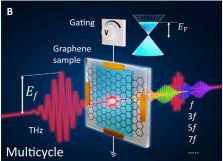
\includegraphics[width=0.8\textwidth]{pic/HHG_intro.pdf}
	\caption[Lab coordinate system]{Schematic of the experimental set-up in Schematic and main results of the THz high-harmonic generation in graphene sample. Electrical tunability of terahertz nonlinearity in graphene ~\cite{kovalev2021electrical}, Copyright 2021, Science Advances. Quasi-monochromatic, linearly polarized THz pump wave from the TELBE source is incident on a graphene sample, single-layer CVD-grown graphene deposited on SiO2 substrate. The incident THz field drives the nonlinear current in graphene, leading to re-emission at higher odd-order harmonics that appear in the spectrum of the transmitted THz signal.}
	\label{fig: HHG_intro}
\end{figure}
Traditional hgh-order harmonic generation (\gls{HHG}) is a phenomenon where intense laser light interacts with a gas, causing the generation of very high-frequency light waves. This process typically occurs when a strong laser field ionizes a material, causing electrons to be ripped away from atoms.
These electrons then undergo complex dynamics, involving acceleration, coherent motion, and recombination with their parent ions. Through this intricate dance, the electrons emit high-energy photons with frequencies much higher than that of the incident laser, often extending into the extreme ultraviolet (XUV) and X-ray regions of the electromagnetic spectrum \cite{gaumnitz2017streaking}.\\
\\
Since first observed in 1987 using rare gases as target specimens \cite{McPherson:87, Ferray_1988},  gas-phase HHG has been intensively utilized to generate ultrashort attosecond light pulses~\cite{PhysRevLett.68.3535, PhysRevLett.70.1599, PhysRevA.49.2117} for investigating ultrafast dynamics in matter in the time domain which is a typical time scale for the motion of electrons.\cite{baltuvska2003attosecond, Goulielmakis2010, doi:10.1126/science.1260311, doi:10.1126/science.aag1268}. HHG provides a unique window into electron dynamics and allows us to investigate processes occurring on attosecond timescales. The emitted harmonics carry valuable information about the electronic structure, band gaps, and transient states of the material, offering a powerful tool for probing and controlling ultrafast processes.
In recent years, there have been significant advancements in experimental techniques for studying high-order harmonic generation. The use of intense femtosecond laser pulses, pulse shaping methods, and advanced detection schemes have enabled precise control and characterization of the generated harmonics. These experimental advances have led to breakthroughs in attosecond science, providing tools for investigating ultrafast phenomena in a wide range of atoms ~\cite{Goulielmakis2010,PhysRevLett.105.143002,PhysRevLett.106.123601}, molecules~\cite{Warrick2016,Reduzzi2016,PhysRevResearch.3.043222}, and solids~\cite{doi:10.1126/science.1260311, doi:10.1126/science.aag1268, Mashiko2016,Siegrist2019, vampa2017merge}.
The HHG in solid-state systems was first observed in ZnO in 2011 in mid-infrared (MIR) laser field~\cite{Ghimire2011}, and it has since garnered significant attention, both from a fundamental research perspective and due to its technological potential, as evidenced by recent studies in solids~\cite{Ghimire2019, Silva2019, Nakagawa2022,gorlach2022high, neufeld2023there}. \textcolor{red}{Figure~\ref{fig: HHG_intro} shows the recent experimental set-up for efficient terahertz high-harmonic generation in graphene ~\cite{hafez2018extremely, kovalev2021electrical}, we will have a detailed theoretical study in Chapter.~\ref{ch:ch4} on it's mechanism.}


%=========================================================================================================================================================
\section{Review on Theoretical Models}
The generation of nonlinear optical response in solids involves complex quantum mechanical processes and intricate
interplays between the laser field and the electronic structure of atoms. The fundamental processes involved in \gls{HHG} in a gaseous medium can
be understood within the framework of the well-known three-step model  \cite{corkum1993plasma,
	lewenstein1994theory}. This semi-classical framework delineates the gas HHG process through three stages, see Figure.~(\ref{fig: 3step}):
\begin{itemize}
	\item 1. Ionization/Tunneling: Initially, an electron is ionized by the intense laser field and electrons are stripped away from the atom due to the strong electric field of the laser.

	\item 2. Acceleration: Subsequently, the strong laser field imparts energy to the liberated electron kinetic energy, propelling its acceleration away from the ionized molecule.

	\item 3. Recombination: In the final step, the oscillatory force of the laser field drives the electron back toward the ionized parent molecule. During this process, the electron undergoes recombination with the molecule, releasing the surplus kinetic energy acquired in the second step in the form of a high-energy photon.\\
\end{itemize}

\begin{figure}[htpb]
	\centering
	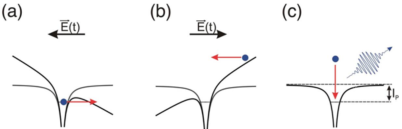
\includegraphics[width=0.9\textwidth]{pic/3step.pdf}
	\caption[Lab coordinate system]{Three step model: (a) Ionization/Tunneling (b) Accelaeration (c) Recombination}
	\label{fig: 3step}
\end{figure}
However, this model is not directly applicable to solid-state HHG due to differences in density, structure, band structure, Coulomb interactions, and surface effects between gases and solids. Solid-state HHG involves more complex mechanisms, including interactions with the crystalline lattice and surface effects, requiring sophisticated theoretical models for accurate description.

The understanding and control of HHG have been greatly advanced by the development of sophisticated
theoretical models, the primary and widely used numerical methods are based on time-dependent
Schrödinger equation (\gls{TDSE}) , semiconductor Bloch equations (\gls{SBE})
and time-dependent density-functional theory (\gls{TDDFT}).
We won't go in detailed about the theoretical foundations, but just summarize current status and some challenges of present numerical simulations which are yet to be improved or solved, for detailed mechanisms and numerical implementations, please refer to the basic references where all those methods are disucssed at lenght.

\begin{itemize}
	\item The time-dependent-Schr\"odinger equation (\gls{TDSE}) model \cite{wu2015high, wu2017orientation, plaja1992high, hawkins2015effect, ndabashimiye2016solid, wu2016multilevel, guan2016high, jin2018high, du2018high}, utilizing both Bloch state basis and Houston state basis, is proficient in examining electronic dynamics within periodic potentials. Nonetheless, simulating the HHG of real solid materials proves challenging, primarily due to the method's reliance on idealized model potentials.
	\item The semiconductor Bloch equations (\gls{SBE}) \cite{hohenleutner2015real, schubert2014sub, langer2016lightwave, vampa2014theoretical, mcdonald2017enhancing, yu2018two, luu2016high, golde2008high, jiang2018role, vampa2015semiclassical, tamaya2016diabatic}, improving it from a two-band model to a multiband model allows for a more comprehensive study of real systems, effectively capturing the main features of High-Order Harmonic Generation (HHG) in solids. This enhancement involves incorporating accurate energy bands and transition dipole moments derived from first-principles calculations. Future endeavors should focus on obtaining the correct phase of transition dipole elements. However, a significant challenge persists as current first-principles codes often yield random phases for transition dipole moments.
	\item The time-dependent density-functional theory (\gls{TDDFT}) model \cite{tancogne2017impact, tancogne2018ultrafast, tancogne2017ellipticity, hansen2017high, meng2018real, floss2018ab, bauer2018high} appears to be the ideal approach for straightforwardly studying High-Order Harmonic Generation (HHG) in solids within real coordinate space. However, its main drawback lies in its significant computational time requirements. Additionally, directly and intuitively analyzing the physical processes or mechanisms within the solid-state energy band picture can pose challenges within the TDDFT framework.
\end{itemize}
Furthermore, properly incorporating Berry curvature in models and understanding its role in solid High-Order Harmonic Generation (HHG) requires more attention in future theoretical simulations. Despite lingering open questions in this evolving field, it's hoped that this review can offer valuable reference points, and ongoing efforts from the relevant community will gradually illuminate the intricacies of solid HHG studies.
%==============================================================================================================================================================================
\section{Structure of the Thesis}
This thesis is organized as follows: Chapter.~\ref{ch:ch2} first introduces the crystallographic discription
for typical hexagonal lattice we are studying, then we study the light-induced electron dynamics in 2D materials based on the tight-binding model by
time-dependent Schrodinger Equation and quantum master equation, to account for dissipative phenomena that plays a fundamental role in the laser induced electron dyanmics that we will describe in detail in the follwoing chapters of this thesis.
In Chapter.~\ref{ch:ch3} we investigate light-induced electron dynamics in monolayer hexagonal
boron nitride under the influence of two-color linearly-polarized laser fields at frequencies
$\omega$ and $2\omega$, by solving the time-dependent Schr\"odinger equation with a tight-binding
model. We start from time-dependent perturbative analysis in the weak field regime, then we expand
our results to third-order nonlinear regime and deeply off-resonant highly-nonlinear regime.
In Chapter.~\ref{ch:ch4}, we study THz-induced HHG in graphene with the method described by quantum
master equation. The microscopic mechanism of
HHG with the quasi-static approximation and the population distribution in the Brillouin zone is
described in detail together with its numerical implementation in Chapter.~\ref{ch:ch5}. We further elucidate the role of the nonequilibrium nature of THz-induced electron dynamics by comparing the nonequilibrium picture in the present work and the thermodynamic picture in the previous work \cite{mics2015thermodynamic}.
We explore the possibility of using a THz
field to enhance MIR-induced HHG in graphene based
on the knowledge gained from Chapter.~\ref{ch:ch4}. We investigate the dynamics under MIR and THz fields and evaluate the emitted harmonic spectra. As a result of the analysis, we find that cou- pling via the induced coherence by THz and MIR fields plays an essential role in enhancing MIR-induced HHG, clarifying the importance of the field-induced coherence beyond the simple population effect.
Finally, the conclusion and perspectvies of this thesis is summarized in in Chapter.~\ref{ch:ch6}
